\documentclass[a4paper,twoside,11pt]{report}
\usepackage[english]{babel}  
\usepackage[utf8]{inputenc} 
\usepackage[T1]{fontenc} 
\usepackage[pdftex,scale={.8,.8}]{geometry}
\usepackage{layout}
\usepackage{fancybox}
\usepackage[pdftex]{graphicx}
\usepackage{fancyhdr}
\usepackage{listings}
\usepackage[parfill]{parskip}
\usepackage{xcolor}
\usepackage{%
  array,
  booktabs,
  dcolumn,
  rotating,
  shortvrb,
  units,
  url,
  lastpage,
  longtable,
  lscape,
  multirow,
  amssymb,
  amsmath,
  float,
  chngpage,
  colortbl,times,
}
\usepackage{hyperref}
\usepackage[toc, nonumberlist, acronym, shortcuts]{glossaries}
\usepackage[toc, page]{appendix}

\usepackage{titlesec}
\usepackage{tikz}
\usepackage{pgfplots}
\usepackage{wrapfig}
\titleformat{\chapter}[hang] 
{\normalfont\huge\bfseries}{\thechapter}{1em}{} 
\titlespacing*{\chapter}{0pt}{0pt}{20pt}
\makeglossaries

\pgfplotsset{compat=1.9}

\usepackage{pdfpages}
\usepackage{fancyhdr}
\usepackage{xfrac}

\definecolor{mygreen}{rgb}{0,0.6,0}
\definecolor{mygray}{rgb}{0.5,0.5,0.5}
\definecolor{mymauve}{rgb}{0.58,0,0.82}

\lstset{
	backgroundcolor=\color{white},
	basicstyle=\footnotesize,
	breakatwhitespace=false,
	breaklines=true,
	captionpos=b,
	commentstyle=\color{mygreen},
	frame=single,
	keepspaces=true,
	keywordstyle=\color{blue},
	numbersep=5pt,
	numberstyle=\tiny\color{mygray},
	rulecolor=\color{black},
	stringstyle=\color{mymauve},
	tabsize=2
}

\newcommand*\NewPage{\newpage\null\thispagestyle{plain}\newpage}


\addto\captionsenglish{
	\renewcommand{\bibname}{List of References}
	\renewcommand{\lstlistlistingname}{List of Listings}
}

\setlength{\headheight}{14pt} 

\loadglsentries{05-glossary.tex}
\loadglsentries{06-acronyms.tex}
\addbibresource{80-references.bib}
\makeglossaries

\begin{document}
\pagenumbering{roman}
\fancypagestyle{plain}{%
  \fancyhead[RO, LE]{\thepage}
  %\fancyhead[RE]{test}
  \fancyhead[LO, RE]{\nouppercase{\leftmark}}
  \fancyfoot{}
  \renewcommand{\headrulewidth}{0.4pt}% Line at the header invisible
}
\begin{titlepage}
    \begin{center}
        \vspace*{1cm}
        
        \Huge
        Wearables in Logistics - Demo Facility
                
        \vspace{1cm}
        \LARGE
        Final report of bachelor thesis
        
        \vspace{5cm}
        Submitted by Lukas Rolle
        
        \vspace{1cm}
        \large
        In fulfilment of the requirements for the degree\\
        Bachelor of Science in Informatics\\
        To be awarded by the\\
        Fontys Hogeschool Techniek en Logistiek
        
        \vfill
        
        \normalsize
        Venlo, \today
        
    \end{center}
\end{titlepage}

\chapter*{Information Page}
\textbf{Student Information} \hfill \vspace{0.3cm} \\
\begin{tabular}{p{0.3\linewidth} p{0.5\linewidth}}
	Name: & Lukas Rolle \\
	Date of Birth: & 23 March 1994 \\
	Place of Birth: & Moers, Germany \\
	Student Number: & 2310309 \\
	Study Course: & Informatics: Software Engineering
\end{tabular}

\textbf{Thesis Information} \hfill \vspace{0.3cm} \\
\begin{tabular}{p{0.3\linewidth} p{0.5\linewidth}}
	Time frame: & 01. February - 30. June 2017 \\
	Date of Delivery: & 28 March 2017
\end{tabular}

\textbf{Company Information} \hfill \vspace{0.3cm} \\
\begin{tabular}{p{0.3\linewidth} p{0.5\linewidth}}
	Name: & Fontys Hogeschool Techniek en Logistiek\\
	Address: & Tegelseweg 255\\
	Postal code: & 5912 BG\\
	City: & Venlo \\
	Country: & Netherlands
\end{tabular}

\textbf{Educational Institution} \hfill \vspace{0.3cm} \\
\begin{tabular}{p{0.3\linewidth} p{0.5\linewidth}}
	Name: & Fontys Hogeschool Techniek en Logistiek \\
	Address: & Tegelseweg 255 \\
	Postal code: & 5912 BG \\
	City: & Venlo\\
	Country: & Netherlands 
\end{tabular}

\textbf{Examination Committee} \hfill \vspace{0.3cm} \\
\begin{tabular}{p{0.3\linewidth} p{0.5\linewidth}}
	Company Supervisor: & Stefan Sobek	\\
	Supervising Lecturer: & Thijs Dorssers \\
	Examinator: & Christiane Holz \\
	External Representative:  & J. Janssen
\end{tabular}
\input{02-preface}
\chapter*{Statement of authenticity}\addcontentsline{toc}{chapter}{Statement of authenticity}
I hereby solemnly declare for this submitted work, that:

\begin{itemize}
	\item I myself wrote this internship report, without the assistance of any third party,
	\item I did not cut and paste any information (text, figures, diagrams, tables,..) from others without appropriate use of quotation marks and direct reference to their work,
	\item I did not re-word the ideas of others without proper and clear acknowledgement,
	\item I did not make use of ideas or suggestions that originated from others and claim these as my own,
	\item I did not include words from other’s work without permission.
\end{itemize}

I am fully aware that any violation of the above will be declared fraud and may result in disadvantageous consequences for me (for example withdrawal of study credits and, in case of a repeated violation, withdrawal of complete study units). If fraud can be proved, I will be required to bear the costs of investigation into and sourcing of the original document.


Name: Lukas Rolle

Place / Date: Venlo, \today


Signature:
\chapter*{Abstract}\addcontentsline{toc}{chapter}{Abstract}
Many small- and medium sized enterprises have difficulties in trying out new technologies, as they often just do not have the needed resources to spend on the newest technology. The LOGwear project aims to give these companies the possibility to stay competitive in that area, it tries to take generalized logistics processes and combines these with wearables and make the results available to everyone.

This thesis is about the creation of a generalized reference model, that allows everyone a head start on creating their own application with a wearable in the area of logistics. Furthermore a demo facility is planned to be created to allow everyone that is interested  in adopting the wearable technology to get hands-on experience. This demo facility is a physical area, where interested can come to visit and get a demonstration of how a process could be improved with the help of wearables. The environment for the demo facility is trying to mock a real world logistics company as closely as possible, using processes from logistics companies as a base.

This should allow companies, that are interested in adopting new technology, to inform themselves about these technologies easily, find technologies they think are interesting for their way of working, see how the technology actually works in a hands-on environment and then make an educated decision if the adoption of a wearable is something that could help improve their own processes.

\vspace{2cm}

Kleine- und Mittelständische Unternehmen haben oft Probleme damit neue Technologien auszuprobieren, da die dazu nötigen Ressourcen oft nicht vorhanden sind um die neuesten Technologien auszuprobieren. Das LOGwear Projekt versucht diesen Unternehmen die Möglichkeit zu geben in dieser Umgebung trotzdem wettbewerbsfähig zu bleiben. Es versucht standardisierte logistische Prozesse zu nehmen und Sie mit Wearables zu verbinden und stellt die Ergebnisse frei zur Verfügung.

Diese Abschlussarbeit beschäftigt sich mit der Erstellung eines standardisierten Referenzmodells, das eine schnellere Erstellung einer eigenen Anwendung mit wearables erlaubt. Weiterhin ist eine Testeinrichtung geplant die kleinen- und mittelständischen Unternehmen die daran interessiert sind, die Möglichkeit gibt  Wearables selbst auszuprobieren. Die Testeinrichtung ist eine Umgebung zu der interessierte gehen können, um selbst sehen oder ausprobieren können ob ein bestimmtes wearable etwas für ihre Unternehmensstruktur ist. Es wird versucht mit der Testeinrichtung die tatsächliche Umgebung eines Logistikunternehmens nachzuahmen, in dem man wirkliche logistische Prozesse als Basis für die Testeinrichtung nimmt.

Damit sollte interesierten Unternehmen erlaubt werden, sich auf einfache Art und Weise über neue Technologien zu informieren, Technologien zu finden die in die Unternehmensprozesse passen könnten, zu sehen wie diese Technologien tatsächlich funktionieren und daraufhin eine informierte Entscheidung zu treffen, ob diese Technologie tatsächlich etwas ist, was Ihre Unternehmensprozesse verbessern könnte.

\tableofcontents\thispagestyle{plain}
\listoffigures\addcontentsline{toc}{chapter}{List of Figures}
\listoftables\addcontentsline{toc}{chapter}{List of Tables}
%\lstlistoflistings
\printglossaries
\cleardoublepage

\fancypagestyle{plain}{%
  \fancyhead[RO, LE]{\thepage}
  %\fancyhead[RE]{test}
  \fancyhead[LO, RE]{\nouppercase{\leftmark}}%\thechapter.\hspace{5pt}
  \fancyfoot{} 
  \renewcommand{\headrulewidth}{0.4pt}% Line at the header invisible
}
\renewcommand{\chaptermark}[1]{%
\markboth{\textbf{#1}}{}}
\pagenumbering{arabic}
\pagestyle{plain}
\chapter{Introduction}
This document is the project plan for the creation of a demo facility for the LOGwear project.

\section{LOGwear}
LOGwear is a research project that aims to bring wearable to the area of logistics, especially to \gls{sme}. It is a German-Dutch project were multiple parties are cooperating to create results in the research project. Involved in this are two Universities of applied sciences, \gls{fhtenl} in Venlo as the Lead-Partner, Netherlands and \gls{hsnr} in Krefeld, Germany.

Further on there are also multiple partner companies involved in the project namely KLG Europe bv, Helmut Beyers GmbH and imat-uve GmbH. These partner companies are there to give the knowledge about logistics processes, as well as to verify and test the results.

The project is backed within the scope of the INTERREG Deutschland-Nederland initiative. It is backed by the \gls{eu}, \gls{mweimh} and the Provincie Limburg as well.

\section{Demo Facility}
The demo facility that should be created for this project will be a physical environment in which a logistics process can be modelled. This process should then be improved by using a wearable. This will be used as a demonstration area for \gls{sme} to see hands-on if a wearable could be used to improve their own processes. The demo facility will be a proof of concept and not a fully implemented solution that could be directly used at a logistics company and instantly work. %This document will inform the user about the LOGwear project in general and more specifically about the task of creating a demo facility for that project and the boundaries of that task.  The demo facility in this is supposed to show the capabilities of a wearable by displaying it is an actual scenario. What this means is a general logistics process is taken and improved with a wearable and then displayed to interested \gls{sme}. It is supposed to be a proof of concept and not a fully implemented solution that could be directly used at a logistics company and instantly work.
\section{Overview}
In this section the following chapters will be shortly explained. 

The first chapter following this, chapter \ref{cha:scope} is about the scope of the assignment as well as the way of working. The risk management done in the project will be explained in chapter \ref{cha:riskManagement}. The last chapter will be about the existing stakeholders in the project \ref{cha:stakeholders}.
\chapter{Context and Scope}\label{cha:context}
This chapter contains the context of the project, including an explanation of the research project LOGwear in section \ref{sec:logwear} and the parties involved in it. Furthermore the general project management strategies will be explained in section \ref{sec:projectManagement}. %Section \ref{sec:referenceArchitecture} and \ref{sec:demoFacility} are explaining the tasks that should be completed during the bachelor thesis. 
Finally, section \ref{sec:planning} is about the time planning and scheduling done for the given project.
\section{LOGwear}\label{sec:logwear}
LOGwear is a research project that aims to bring wearables to the area of logistics, especially to \gls{sme}. It is a German-Dutch research project were multiple parties are cooperating to create results. Involved in this are two Universities of applied sciences, \gls{fhtenl} in Venlo as the lead partner, Netherlands and \gls{hsnr} in Germany.

Further on there are also multiple partner companies involved in the project, namely KLG Europe bv, Helmut Beyers GmbH and imat-uve GmbH. These partner companies are there to give the knowledge about logistics processes, as well as to verify and test the results.

The project is backed within the scope of the INTERREG Deutschland-Nederland initiative. It is backed by the \gls{eu}, \gls{mweimh} and the Provincie Limburg as well. The official kickoff meeting for logWear was in september 2016 and the project will run until march 2018. 

The LOGwear project is consisting of three main \gls{wp}s. \citep{website:logwear}
\begin{description}
	\item[Knowledge Base (\gls{wp}1)] \hfill \\
		The knowledge base is a platform that allows to exchange information between logistics companies which wearable can be used for which process. \citep{bachelorThesis:oliver} \citep{bachelorThesis:sascha}
	\item[Reference Architecture / Reference Model (\gls{wp}2)] \hfill \\
		The expected result for \gls{wp} 2 used to be a reference architecture, this has internally changed to a reference model, the differences about these two and what is expected from the reference model can be found in chapter \ref{cha:reference}. 
	\item[Demo Facility (\gls{wp}3)] \hfill \\
		The demo facility is the creation of a physical demo that allows \gls{sme} to see the benefits of wearables for a demo process. The difference between the demo facility created during this thesis and \gls{wp} 3 is, that the \gls{wp} 3 is the implementation of a wearable solution at a pilot company, while the demo facility created during this thesis is in an enclosed environment that does not need to follow all constraints of deploying something at a company. Further details for the demo facility are described in chapter \ref{cha:demoFacility}. 
\end{description}
%\section{Reference Model}\label{sec:referenceArchitecture}
The task to create a reference model was one of the three big work packages that are existing in the LOGwear project. \textcolor{red}{\cite{•}} 
%\section{Demo Facility}\label{sec:demoFacility}

\section{Project Management}\label{sec:projectManagement}
This section contains information about the project management details during the project.
\newpage
\subsection{Stakeholder}
Stakeholder Management involves identifying parties that are involved in the project. This ranges from people that are actively part of the development of the project or companies that might be interested in the end result. In the table \ref{tab:stakeholder} the most important stakeholders can be found. The stakeholders will themselves will be further explained in sections \ref{sssec:internalStakeholders}, which will explain the internal stakeholders, and \ref{sssec:externalStakeholders} will explain the external stakeholders involved in the project.
\begin{table}[htbp]
\centering
\resizebox{\textwidth}{!}{
\begin{tabular}{|p{.04\textwidth}|p{.22\textwidth}|p{.115\textwidth}|p{.118\textwidth}|p{.1\textwidth}|p{.085\textwidth}|p{.16\textwidth}|}
\hline
\textbf{Nr} & \textbf{Stakeholder} & \textbf{Company / Institution} & \textbf{Internal / External} & \textbf{Level of Interest} & \textbf{Level of Influence} & \textbf{Potential management strategies} \\ \hline
1  & Employer             & \gls{fhtenl}        & Internal            & Medium            & High               & Keep Satisfied            \\ \hline
2  & Student Workers      & \gls{fhtenl}        & Internal            & Medium            & Low                & Keep Informed             \\ \hline
3  & Graduation Student   & \gls{fhtenl}        & Internal            & High              & High               & Key Player                \\ \hline
4  & Project Manager      & \gls{fhtenl}        & Internal            & High              & High               & Key Player                \\ \hline
5  & Company Supervisor   & \gls{fhtenl}        & Internal            & High              & High               & Key Player                \\ \hline
6  & Project Team         & \gls{fhtenl}        & Internal            & High              & High               & Key Player                \\ \hline
7 & Partner University   & \gls{hsnr}          & External            & Medium              & Low                & Keep Informed             \\ \hline
8  & Pilot Company        & KLG                   & External            & High              & High               & Key Player                \\ \hline
9  & Examiner             & \gls{fhtenl}        & External            & Low               & High               & Keep Satisfied            \\ \hline
10  & Supervising Lecturer & \gls{fhtenl}        & External            & Medium            & Low                & Keep Informed             \\ \hline
\end{tabular}
}
\caption{Stakeholder Register}
\label{tab:stakeholder}
\end{table}

Figure \ref{fig:stakeholder} can be used to visualize the importance of the stakeholders. The color is used to emphasize the importance that this stakeholder is properly managed.

\begin{figure}[htbp]
	\centering
	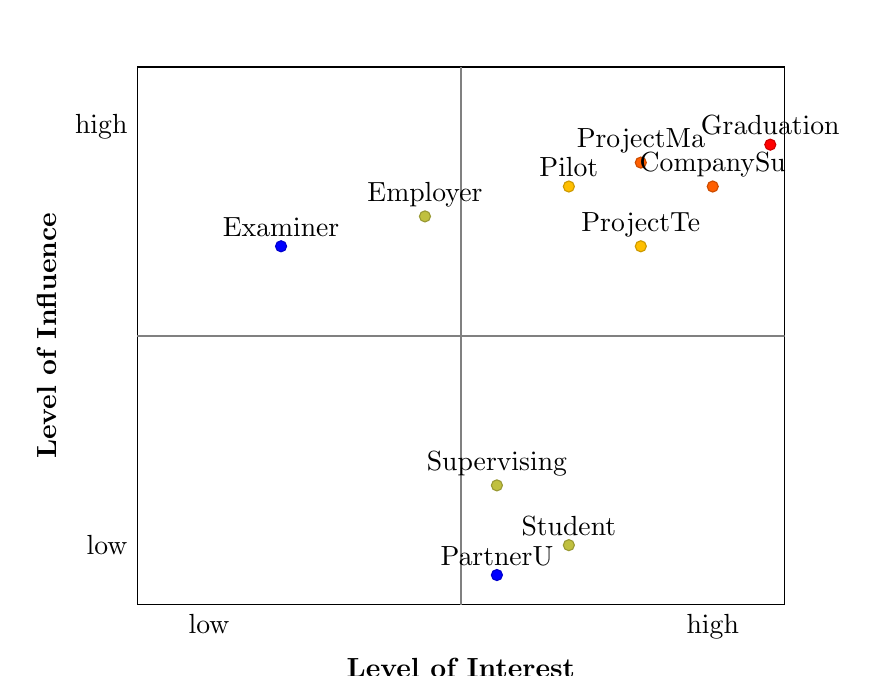
\begin{tikzpicture}
		\begin{axis}[
			scale=1.2,
			xmin=1,
			xmax=10,
			ymin=1,
			ymax=10,
			xtick,
			ytick,
			extra x ticks={2,9},
  			extra x tick labels={low, high},
  			xtick style={draw = none},
  			extra y ticks={2,9},
  			extra y tick labels={low, high},
			ytick style={draw = none},
			xlabel=\textbf{Level of Interest},
			ylabel=\textbf{Level of Influence},
			x
			]
			\addplot[
			scatter,
			only marks,
			nodes near coords*={\myvalue},  
			point meta=\thisrow{color},
			visualization depends on={value \thisrow{myvalue} \as \myvalue},
			] table[x=x, y=y]
			{
			x	y	color	myvalue
			5	7.5	2	Employer
			7	2	2	Student Workers
			7	8	3	Pilot Company 
			3	7	1	Examiner
			6	3	2	Supervising Lecturer
			9.8	8.7	5	Graduation Student 
			8	8.4	4	ProjectMa 
			9	8	4	CompanySu 
			8	7	3	ProjectTe 
			6	1.5	1	PartnerU
			};
			\addplot[gray,thick, no markers] coordinates {(1,5.5) (10,5.5)};
			\addplot[gray,thick, no markers] coordinates {(5.5,1) (5.5,10)};
		\end{axis}
	\end{tikzpicture}
	\caption{Stakeholder Graph}
	\label{fig:stakeholder}
\end{figure}
\subsubsection{Internal Stakeholders}\label{sssec:internalStakeholders}
Internal Stakeholders are parties that are a part of the team that is working directly on the project in one way or the other. In this section, the internal stakeholders mentioned in table \ref{tab:stakeholder} will be listed again and explained.

\begin{description}
	\item[Employer] \hfill
	
	The employer in this project is an institution and not a single person. This does not change the fact, that the employer is interested in the project, as he is financing the project. Also the employer could change the outcome, if he is not accepting the proposed plans. It is important, that this party is kept satisfied as more work could be created when the plan has to change.
	\item[Student Workers] \hfill
	
	Student Workers are employed to help in the LOGwear project in general. While they currently are not involved with the process of the creation of the demo facility that might change in the future, therefore they should be kept informed.
	\item[Graduation Student] \hfill
	
	The graduation student is the person mainly responsible for the development of the demo facility and therefore has a lot of responsibility and interest towards the project.
	\item[Project Manager] \hfill
	
	The project manager is responsible for the general planning of the project. Planning meetings with the different parties and coordinating them.
	\item[Company Supervisor] \hfill
	
	The company supervisor is looking over the progress of the graduation student and is giving advice if needed. 
	\item[Project Team] \hfill
	
	The project team are the members of the team actively developing the application prototype and are involved in building the demo facility afterwards.
\end{description}

\subsubsection{External Stakeholders}\label{sssec:externalStakeholders}
External Stakeholders are parties that are involved in the project, but are not a part of the team actively developing the project. In this section, the external stakeholders mentioned in table \ref{tab:stakeholder} will be listed again and explained.

\begin{description}
	\item[Partner University] \hfill
	
	The partner university is also working on the LOGwear project, but on a different aspect. They might be interested in project of creating a demo facility, but probably will not interfere with it.\\
	
	\item[Pilot Company] \hfill
	
	The pilot company involved is the logistics company KLG. They bring in the highest amount of domain knowledge and are interested in the project to improve their own processes. They could influence the project easily by not approving the planned demo facility due to problems with how the logistics process is modelled.
	\item[Examiner] \hfill
	
	While the examiner is not involved in the project itself, the examiner will finally assesses the performance of the graduation student.
	\item[Supervising Lecturer] \hfill
	
	The supervising lecturer is there to answer questions and support the student from a software engineering standpoint. While not having a lot of influence on the project itself, the supervising lecturer is interested in what the student is doing and especially how he is doing it.
\end{description}
\newpage
\subsection{Risks}
Risk management is about identifying risks and finding solutions to problems before they can occur. The list of risks can be found in table \ref{tab:RiskRegister}. The identified risks will increase as the project moves forward. Especially when a decision is made for the wearable and the process. 

\begin{table}[htbp]
\centering
\footnotesize
\resizebox{\textwidth}{!}{
\begin{tabular}{|>{\raggedright\arraybackslash}p{.03\textwidth}|>{\raggedright\arraybackslash}p{.1\textwidth}|>{\raggedright\arraybackslash}p{.2\textwidth}|>{\raggedright\arraybackslash}p{.08\textwidth}|>{\raggedright\arraybackslash}p{.08\textwidth}|>{\raggedright\arraybackslash}p{.15\textwidth}|>{\raggedright\arraybackslash}p{.13\textwidth}|>{\raggedright\arraybackslash}p{.11\textwidth}|}
\hline
\textbf{Nr} & \textbf{Risk Name}                                    & \textbf{Description}                                                                                                      & \textbf{Prob-ability} & \textbf{Impact} & \textbf{Root Cause}                                                                                       & \textbf{Potential Responses}                                              & \textbf{Risk Owner} \\
\hline
1           & Wearable unavailable          & The wearable desired to be used in the demo facility is unavailable.                                                      & Low                  & Medium          & The desired product is a prototype or similar.                                                            & Choosing a different wearable that is already readily available.          & Graduation Student  \\ \hline
2           & Demo Area & A demo area is in mind that could potentially be rented, but that could not be possible.                                  & Medium               & Medium          & The owner of the place does not rent the area.                                                            & Researching possible places where the demo facility could be created.     & Graduation Student  \\ \hline
3           & Unusable wearable             & A wearable is chosen that does not have the capabilities to fulfill the things that were planned with the demo facility.  & Low                  & High            & Too little research done on the wearables, or the researched material was wrong.                          & Altering the demo scenario to accommodate the problems with the wearable. & Graduation Student  \\ \hline
4           & Vocabulary unclear            & The vocabulary used in the logistics branch, especially abbreviations and acronyms might cause problems in communication. & High                 & Low             & The graduation student has too little knowledge of the logistics branch, at the beginning of the project. & Asking questions if a word's or sentence's meaning is not clear.          & Graduation Student. \\ \hline
\end{tabular}
}
\caption{Risk Register}
\label{tab:RiskRegister}
\end{table}

\begin{wrapfigure}{l}{0pt}
	\centering
	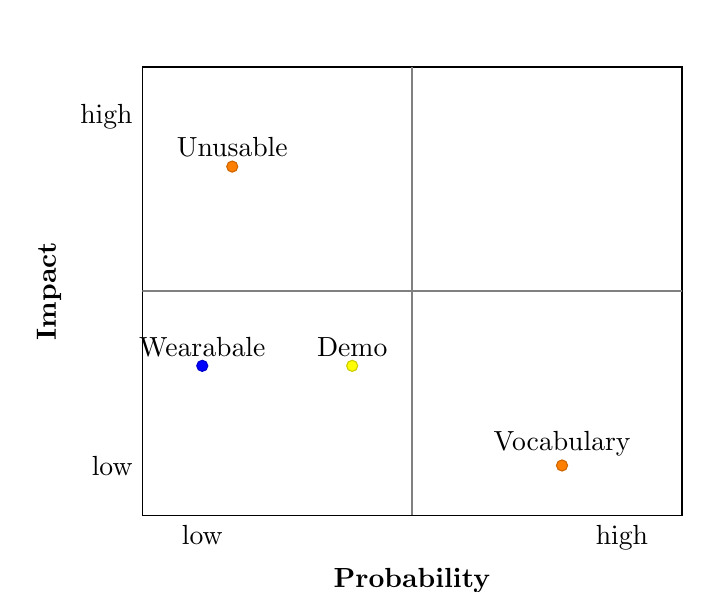
\begin{tikzpicture}
		\begin{axis}[
			scale=1,
			xmin=1,
			xmax=10,
			ymin=1,
			ymax=10,
			xtick,
			ytick,
			extra x ticks={2,9},
  			extra x tick labels={low, high},
  			xtick style={draw = none},
  			extra y ticks={2,9},
  			extra y tick labels={low, high},
			ytick style={draw = none},			
			xlabel=\textbf{Probability},
			ylabel=\textbf{Impact},
			x
			]
			\addplot[
			scatter,
			only marks,
			nodes near coords*={\myvalue},  
			point meta=\thisrow{color},
			visualization depends on={value \thisrow{myvalue} \as \myvalue},
			] table[x=x, y=y]
			{
			x	y	color	myvalue
			2	4	1	Wearabale
			4.5	4	2	Demo
			2.5	8	3	Unusable
			8	2	3	Vocabulary
			0	0 	4
			};
			\addplot[gray,thick, no markers] coordinates {(1,5.5) (10,5.5)};
			\addplot[gray,thick, no markers] coordinates {(5.5,1) (5.5,10)};
		\end{axis}
	\end{tikzpicture}
	\caption{Risk Graph}
	\label{fig:risks}
\end{wrapfigure}

In figure \ref{fig:risks} the risks can be seen in a graph that shows their Probability and Impact again. The color emphasizes the amount of attention a risk should get, in order for the project to continue smoothly.

\cleardoublepage

\subsection{Requirements}
Requirements are for the demo facility only, as the reference model is not an actual product to have any requirements for. Of the current state the demo facility only has few requirements as the wearable is not chosen at this point and only the process is known.

\begin{table}[htbp]
\begin{tabular}{c}

\end{tabular}
\caption{Requirements}
\label{tab:requirements}
\end{table}
\subsection{Quality Management}
Metrics used to determine the quality of the project:

\begin{itemize}
	\item code coverage
	\item language conventions
	\item documentation
	\item possibly performance testing (as wearables tend to be not as powerful focus on performance might not be wrong)
	\item integration testing
	\item code reviews(?)
\end{itemize}
\subsection{Definition of Done}
A part of the software project is done, when it is fully designed, implemented and tested. When that part of the application is passing all of these criteria it is added to a repository where the result is build. When that build is successful that part of the application is done, for the moment. When that part needs to be changed in the future the same procedure will be used again.
\section{Planning}\label{sec:planning}
The initial schedule for the project can be seen in table \ref{tab:schedule}. It is to be mentioned, that the schedule is subject to change as the project goes on. The project will be executed in a scrum-like way that is adapted to the group, given the group size of two developers.
\begin{table}[htbp]
\centering
\large
\resizebox{1\textwidth}{!} {
\begin{tabular}{|c"cc:cccc:cc:ccccccccc:ccc:c|} \hline
\textbf{Sprints} & \multicolumn{2}{>{\centering\arraybackslash} m{.15\textwidth}|}{\textbf{Logistics Processes \& Wearables}} & \multicolumn{4}{>{\centering\arraybackslash} m{.35\textwidth}|}{\textbf{Reference Architecture}} & \multicolumn{2}{>{\centering\arraybackslash} m{.25\textwidth}|}{\textbf{Research Demo Facility}} & \multicolumn{9}{c|}{\textbf{Demo Facility Design and Implementation}}                   & \multicolumn{3}{>{\centering\arraybackslash} m{.25\textwidth}|}{\textbf{Creation Demo Facility}} & \multicolumn{1}{>{\centering\arraybackslash} m{.08\textwidth}|}{\textbf{Buf-fer}} \\ \thickhline
Date                 & 06.02              & 13.02              & 20.02                & 27.02                & 06.03         & 13.03        & 20.03        & 27.03 & 03.04 & 10.04 & 17.04 & 24.04 & 01.05 & 08.05 & 15.05 & 22.05 & 29.05 & 05.06         & 12.06        & 19.06        & 26.06                             \\
Week                       & 6                  & 7                  & 8                    & 9                    & 10            & 11           & 12           & 13    & 14    & 15    & 16    & 17    & 18    & 19    & 20    & 21    & 22    & 23            & 24           & 25           & 26 \\\hline       	              
\end{tabular}
}
\caption{Schedule}
\label{tab:schedule}
\end{table}

The schedule is divided in work packages that are to be executed, it is to be noted, that each work package could be split into multiple sprints in the future. In the following subsections the work packages will be explained.

\subsection{Logistics Processes \& Wearables}
This work package includes research about the gives processes and wearables in general, as well as already choosing potential wearables that could be used to improve the process. The end result for this should be a decision on process and wearable. But the result for this could potentially take longer than this task is scheduled. The wearables should be ranked after getting hands-on experience on them, therefore some of them have to be ordered first.

\subsection{Reference Architecture}
A reference architecture should be created for a sample wearable application. What this work package contains is, the creation of diagrams which show the communication from a wearable to the \gls{wms} or something similar. What should not be created is a full reference architecture for a process that is implemented with a concrete wearable. 

It is about creating the always needed layers when using a wearable in a way that supports most wearable solutions.

\subsection{Research Demo Facility}
This task includes researching what physical objects and what systems would be needed to create a demo facility that could showcase a single process with a single wearable. This also includes the gathering of knowledge of where the demo facility should be created and where to get the needed objects.

\subsection{Demo Facility Design and Implementation}
The work package includes the creation of the software design and implementation for the wearable and all aspects that are needed to fully showcase a process.

\subsection{Creation Demo Facility}
This task includes the physical creation of the demo facility. This means setting up shelves with packages to scan and put on a hand pallet truck. Setting up barcodes on the packages to scan. Setting up an environment that can showcase what is happening better to an audience.

\chapter{Research}\label{cha:research}
This chapter includes the general research that has been done for the project. Which includes the research about some given processes and wearables that could be appropriate for the processes. The CASE Tools chosen at the current state of the project will also be discussed and what they are used for.

\section{Processes}\label{sec:processes}
There were process already modelled and made available in the LOGwear project. The given processes were:

\begin{itemize}
	\item Order Picking High Rack
	\item Order Picking W3-5
	\item Goods Receipt and Put away
\end{itemize}

Those three processes can also be found in \ref{appendix}.

Order Picking High Rack has been discarded due to the nature of what should be created. A simulation that should model a real environment. Modelling a High Rack and usage of that would be too hard and would take too much time.

Goods Receipt and Put away was another process to be considered, but was discarded. The modelling of it would be problematic due to the time delays in the tasks. Furthermore the process showed less potential for improvements with wearables.

Order Picking W3-5 was the process chosen to improve with wearables as multiple possibilities to improve the process were discovered. Also the processes seemed rather easy to model with a demo facility by setting up one or two racks and placing multiple packages on there.

The process has been decided together with the company supervisor.

\section{Wearables}\label{sec:wearables}
Researching wearables was a more problematic task, as the amount of wearables that could be used potentially is a lot higher. Some criteria were set in place for a wearable to be considered in the first place. A wearable has to be either already available, or freely available to order in europe from a trusted source. This leads to well known wearables like the Google Glass to be not even considered as they are not publicly available.


\section{CASE Tools}\label{sec:caseTools}
The \gls{case} tools chose here are only for the parts already decided on. As a chosen wearable could introduce a lot more \gls{case} tools to the project. 
\chapter{Reference Model}\label{cha:reference}
The \gls{reference model} of the LOGwear project is a model that shows how the communication from a wearable to the \gls{wms} or some other system might work. This does not mean that every communication necessarily needs to look like displayed in the \gls{reference model}, but that in general every wearable is able to communicate with an underlying system in the way it is displayed.
The model can be seen in figure \ref{fig:referenceModel}.
\begin{figure}[htbp]
	\includegraphics[width=\linewidth]{images/PackageModel_ReferenceArchitecture}
	\caption{Reference Model LOGwear}
	\label{fig:referenceModel}
\end{figure}

\section{Definition}
A \gls{reference model} is an abstract design used to help others understand the general concept and the relationships between existing entities of a specified environment. Furthermore a \gls{reference model}, in general, does not model anything with a specific technology in mind and rather models everything as general as possible. This is done so that when creating an architecture around the \gls{reference model}. The \gls{reference model} can be used as a template to start working with. Not as a constraint, that holds the architects back. When implementing the \gls{reference model} with a specific technology, it is needed to change existing parts or add new parts to fit the given constraints. A \gls{reference model} as is, is not directly implementable due to the abstract nature.

The aim for a \gls{reference model} is to standardize the way how developers in the future implements an application in the given domain, regardless of the used technologies.\cite{website:oasis-rm}

\section{Design}
As can be seen in figure \ref{fig:referenceModel} the \gls{reference model} is divided into three different packages that all fulfil different responsibilities. First it will be described what this \gls{reference model} can help to create. Therefore the general thought behind the whole model will be explained and afterwards the three packages \texttt{system}, \texttt{communication} and \texttt{wearable} will be explained on their own.

The concept is simple, a wearable is connected to a communication layer, that then again connects to a system, that could be anything, as long as it has an \gls{api}. The arrows are not indicating an information flow but rather an instruction flow. The box that the arrow leaves does invoke an instruction in the box that the arrow points to. The sources of information are generally the \texttt{InputInterfaces}, and the incoming information is spread from there. Depending on the incoming information, actions are invoked. 

The \gls{reference model} is purposely minimalistically designed, to allow most infrastructures and wearables, to apply the model, with as few changes as possible. If for example a new \gls{wms} was used the only component that needs to be changed is the \texttt{SystemConnector} in the \texttt{communication} package. In that case, the wearable that are in use, can also continue to work, just like they normally would, without the need for a new version to be deployed on all of them.

\subsection{Wearable}
The \texttt{\gls{wearable}} package is representing the actual physical wearable, or a set of wearables, that a worker is using. This could be either \gls{smartglasses}, \gls{smartwatch}es, a ring-scanner or some other \gls{wearable}. It could also be a combination of wearables that is used in order to fulfil a certain task. In such cases it is still possible to stick to the \gls{reference model} either by changing the existing model, with multiple \texttt{BusinessLogic} classes in the different wearable and a manager that could handle that. Or it could be, that even when using multiple wearables at once, a single wearable is handling the business logic of all wearables. Then the other wearables could be addressed by just their input- and output- interfaces.

Further on the wearable package is again held as simple as possible. The \texttt{InputInterfaces} are there to get information from the outside world and the \texttt{OutputInterfaces} are there to somehow represent information to the outside world. The \texttt{BusinessLogic} is there to process the incoming data and invoke the appropriate actions, that could be either displaying some information to the user or making a call to the underlying system through the \texttt{CommunicationInterface}.

The \texttt{CommuncationInterface} is the means of communication with an outside computer source, this could be radio, bluetooth, \gls{rest} via \gls{wlan} or some other way of communication. The \texttt{WearableCommunicator} in the \texttt{Communication} package just needs to be able to receive and understand the messages.
\subsection{Communication}
The \texttt{communication} package is existing due to the different technologies used from \gls{wearable}s to connect to other computing devices. The communication layer might also be the only place, where information can be fully controlled by the developer, this is especially interesting when the \texttt{system} is controlled by a third-party. Also needed actions can be taken, if the incoming data has to be transformed into a different format, before either the \texttt{\gls{api}} or the \texttt{wearable} can understand it. 

The \texttt{communication} package could potentially be removed, if the wearable has the needed technology in place to directly connect to the \gls{api} of the given system. But this is in general not recommended, as the communication layer allows the developer to create a more standardized flow of information.

\subsection{System}
The \texttt{system} package here can be something like a \gls{wms} of the company. A system that is mostly a black box with an \gls{api} and a database. Most of the time, the \texttt{system} cannot be changed by the developer, therefore the developer needs to use the possible ways to connect to the given \gls{api}.


\section{Problems}
The main problem that occurred during the creation of the \gls{reference model} was a problem in communication, regarding the names of \gls{reference model} and \gls{reference architecture}. 
\chapter{Demo Facility}\label{cha:demoFacility}
\section{Infrastructure}
\section{Design}
\section{Planning}
\chapter{Conclusion}\label{cha:conclusion}
The reference model is the only current deliverable really created up to this point. This is due to the reference model being a crucial point of the research project. As the research goes on the reference model will be used as the artifact that is used to show developers on how a wearable system should look like in a logistics environment. Therefore the design went through multiple iterations to allow it to fit as many use-cases as possible, while reducing the need to change a lot of the design for each use-case.

The design of the reference model, even though a few communicational problems arose with what was actually expected from it, was successful and the involved parties are happy with how it turned out.

\section*{Further Planning}
Now that the design of the reference model is at a stable state, it can be started to implement the parts of it that are not directly relying on the wearable itself. The wearables will be tested as they become available and a decision will be made depending on the results from that testing. Once that is done, the further creation of the demo facility will be able to planned accordingly and implementation of that can start.

When the creation of the demo facility is finished it is planned to invite \gls{sme}s to test out the wearables and how they could improve their processes.
\printbibliography
\begin{appendices}
\addtocounter{chapter}{1}
\fancypagestyle{plain}{%
  \fancyhead[LO, RE]{\nouppercase{\rightmark}}
}
\renewcommand{\sectionmark}[1]{%
\markboth{\textbf{#1}}{}}

\section{Order Picking Process}
\vspace*{-2cm}
\begin{figure}[H]
	\includegraphics[width=\textwidth, page=1]{images/OrderPickingW3-5}
	\caption{Order Picking Process Diagram \citep{image:logwearOrderPicking}}
	\label{fig:orderPickingProcessDiagram}
\end{figure}
\begin{figure}\ContinuedFloat
	\includegraphics[width=\textwidth, page=2]{images/OrderPickingW3-5}
	\caption*{Figure \ref{fig:orderPickingProcessDiagram}: Order Picking Process Diagram \citep{image:logwearOrderPicking}}
\end{figure}
\begin{figure}\ContinuedFloat
	\includegraphics[width=\textwidth, page=3]{images/OrderPickingW3-5}
	\caption*{Figure \ref{fig:orderPickingProcessDiagram}: Order Picking Process Diagram \citep{image:logwearOrderPicking}}
\end{figure}
\begin{figure}\ContinuedFloat
	\includegraphics[width=\textwidth, page=4]{images/OrderPickingW3-5}
	\caption*{Figure \ref{fig:orderPickingProcessDiagram}: Order Picking Process Diagram \citep{image:logwearOrderPicking}}
\end{figure}

\clearpage

\section{Use Cases Reference Model} \label{sec:useCasesReferenceModel}

\begin{figure}[htbp]
	\begin{UseCase}{UC-W1}{Get Order (Voice)}{Wearable}{1.0}{LUR}
		\Actors{Picking Worker}
		\Description{A picking worker equipped with a wearable is using a voice command to get the next order displayed.}
		\Preconditions{The wearable has to be equipped with an Input Interface accepting voice and and an Output Interface that is able to return information to the user.}
		\Scenario{
			\vspace{0.1\baselineskip}
 		   \begin{enumerate*}
    			\item The Picking worker gives the voice command "Next Order".
    			\item The Wearable asks the WMS for the next order for the specific worker.
    			\item The WMS sends the Data to the Wearable
    			\item The Wearable displays the Data to the order picker.
			\end{enumerate*}
		}
		\Extensions{
			\vspace{0.1\baselineskip}
			\begin{enumerate*}
				\item[-]
			\end{enumerate*}
		}
		\Exceptions{
			\vspace{0.1\baselineskip}
			\begin{enumerate*}
				\item[1.1] The Voice command could not be properly understood. The Wearable does nothing.
				\item[1.2] The Order Picker is already on an Order and that one is unfinished, the command is ignored.
				\item[1.3] Another Voice command is understood, that one is executed.
				\item[3.1] The WMS did not find a next order. The order picker is informed about that.
				\item[4.1] There is an error in the format that was received. The data that could be understood is still displayed and the order picker is informed, that there might be an error with the order.
			\end{enumerate*}
		}
		\Result{The Order Picker has received the next order.}
	\end{UseCase}
	\caption{Use Case: Get Order(Voice)}
\end{figure}

\begin{figure}[H]
	\begin{UseCase}{UC-W3}{Order Control}{Wearable}{1.1}{LUR}
		\Actors{Picking Worker}
		\Description{A picking worker is in the process of picking his order.}
		\Preconditions{The wearable has a vision interface or is in another way able to control what the order picker is doing. Furthermore the order picker is currently in the process of picking an order and is picking a specific item of that order.}
		\Scenario{
			\vspace{0.1\baselineskip}
    		\begin{enumerate*}
    			\item The order picker scans an item.
		    	\item The wearable checks what is being packed.
		    	\item The order picker is putting the item on his hand pallet truck.
		    	\item The wearable is counting the amount of items put onto the hand pallet truck.
		    	\item The order picker scans a new item.
	 		   	\item The wearable detects a new item and ends the counting process for the last item.
	 		   	\item The wearable informs the order picker that everything went correctly with the last item.
    		\end{enumerate*}
		}
		\Extensions{
			\vspace{0.1\baselineskip}
			\begin{enumerate*}
				\item[6.1] When the order has no next item, the worker tries to confirm the order and the wearable can then proceed to check if the amount of picked parcels was correct.
			\end{enumerate*}
		}
		\Exceptions{
			\vspace{0.1\baselineskip}
			\begin{enumerate*}
				\item[7.1] The order picker could have counted wrongly and the wearable is informing him about it. After the order picker has checked the quantity on the Truck, go back to 1. with the item started with.
				\item[7.2] The wearable could have counted wrongly and the wearable is informing the order picker as if he counted wrong. The order picker can check the hand pallet truck for the item and confirm the right quantity.
				\item[7.3] The order picker could have picked the wrong quantity and the wearable could have counted wrong, resulting in the wearable saying the order picker has picked the right amount. An error is made.
			\end{enumerate*}
		}
		\Result{The Order Picker completed a part of the order and the wearable confirmed the quantity of that part.}
	\end{UseCase}
	\caption{Use Case: Order Control}
\end{figure}

\section{Web Application Mockups}\label{sec:webappmockups}
\begin{figure}[htbp]
	\includegraphics[width=\textwidth, page=1]{images/WebAppMockups}
	\caption{Mockup Worker Login}
\end{figure}
\begin{figure}
	\includegraphics[width=\textwidth, page=2]{images/WebAppMockups}
	\caption{Mockup No Order Started}
\end{figure}
\begin{figure}
	\includegraphics[width=\textwidth, page=3]{images/WebAppMockups}
	\caption{Mockup Start Order}
\end{figure}
\begin{figure}
	\includegraphics[width=\textwidth, page=4]{images/WebAppMockups}
	\caption{Mockup Confirm Order Line}
\end{figure}
\begin{figure}
	\includegraphics[width=\textwidth, page=5]{images/WebAppMockups}
	\caption{Mockup Confirm Order}
\end{figure}
\end{appendices}

\end{document}